\section{Experiments}


\subsection{Baselines}
\begin{table}[t]
    \centering
    \renewcommand{\arraystretch}{1.0}
    \begin{tabular}{lcccc}
        \toprule
         & \multicolumn{2}{c}{English} & \multicolumn{2}{c}{German} \\
         & I $\rightarrow$ T & T $\rightarrow$ I & I $\rightarrow$ T & T $\rightarrow$ I\\
         \midrule
         En & 40.5  &  28.8 & 34.9 & 24.6  \\
         \; + De & 41.4 & 29.9  & \textbf{38.6} & 26.0\\
         \; \; + c2c & \textbf{42.8} & \textbf{32.1} & 38.3 & \textbf{27.7} \\
         \bottomrule
    \end{tabular}
    
    \caption{Recall @ 1 Image-to-Text and Text-to-Image baseline results for models trained on only the Multi30K German, German + English, and with the additional caption--caption ranking objective.}\label{tab:baseline}
\end{table}

Table \ref{tab:baseline} shows our reproduction of the baselines of \citet{kadar2018conll}. We trained the models on only the in-domain English and German Multi30K data. We see that for both languages, the best performance (excluding R@1 image--text retrieval in German) is achieved by training a model on the bilingual data with the caption--caption ranking objective. The numbers we report are overall slightly higher than those reported in \citet{kadar2018conll}, which we attribute to using different random seeds. 


\subsection{Domain-shift: Training with COCO}

Tables \ref{tab:coco_en} and \ref{tab:coco_en_in_de} show the results of training the model with an additional out-of-domain captioned images dataset. We use the COCO dataset, which contains 82,783 images, each of which is paired with five captions, giving a total of 413,915 extra image--sentence pairs. 

Table \ref{tab:coco_en} shows that the performance of an English model that is only trained on the COCO data is substantially below a model only trained on Multi30K English data (Line 3 compared to Line 1). This implies that there is a domain-shift between the COCO and the Multi30K datasets that cannot be overcome by training on the larger and broader-domain COCO data. We also see that the English models benefit from training with the COCO data in addition to the Multi30K English data. The best text-to-image and image-to-text retrieval performance is found for the model trained on the COCO + English + German + c2c (Line 6). Nevertheless, comparing Line 2 against Lines 4--6, it is clear that training on the Multi30K English and the COCO data is consistently 5--6 Recall @ 1 better than the best-performing baseline model. We speculate that this is because training on both English data sets results in better word embeddings for the English examples, as opposed to also updating the mostly separate word embeddings for the German portion of the Multi30K data.

Table \ref{tab:coco_en_in_de} shows the results for German. These models only benefit from training on the COCO data when we also train with all the Multi30K data and the c2c objective. Performance drops if we only train on the the out-of-domain COCO data and the German in-domain data, which further supports our claim that there is a domain shift between the datasets because it improved the German baselines in Table \ref{tab:baseline} to also train on the in-domain English Mutli30K data.

\begin{table}[]
    \centering
    \renewcommand{\arraystretch}{1.0}
    \begin{tabular}{rlcc}
        \toprule
         & & I $\rightarrow$ T & T $\rightarrow$ I \\
         \midrule
         1 & En & 40.5 & 28.8 \\
         2 & En + De + c2c & 42.8 & 32.1 \\
         \hdashline         
         3 & COCO & 34.4  & 24.8 \\
         4 & \; + En & 46.2 & 33.4   \\
         5 & \; + En + De & 46.0  & 33.6  \\
         6 & \; + En + De + c2c & \textbf{46.5} & \textbf{34.8} \\         
         \bottomrule
    \end{tabular}
    \caption{Recall @ 1 for English models trained with the out-of-domain English COCO dataset. We also include a subset of the baseline models for ease-of-comparison.}\label{tab:coco_en}
\end{table}

\begin{table}[]
    \centering
    \renewcommand{\arraystretch}{1.0}
    \begin{tabular}{rlcc}
        \toprule
         & & I $\rightarrow$ T & T $\rightarrow$ I \\
         \midrule
         1 & De + En + c2c & 38.3 & 27.7 \\
         \hdashline
         2 & COCO + De & 36.4 & 25.7\\
         3 & \; + En & 39.2 & 27.1   \\
         4 & \; + En + c2c & \textbf{40.6} & \textbf{28.8} \\
         \bottomrule
    \end{tabular}
    \caption{Recall @ 1 results for German models trained with the out-of-domain English COCO dataset. We include the best-performing baseline from Table \ref{tab:baseline}.}\label{tab:coco_en_in_de}
\end{table}

\subsection{Training with pseudo-paired COCO data}

\begin{table}[]
    \centering
    \renewcommand{\arraystretch}{1.0}
    \begin{tabular}{rlcc}
        \toprule         
        & & I $\rightarrow$ T & T $\rightarrow$ I \\
        \midrule
        1 & COCO + En + De + c2c & 46.5 & 34.8 \\         
        \hdashline
        %3 & \; \; + c2c &  \textbf{47.7} & \textbf{35.3} \\
        %5 & \; \; + c2c & 47.5 & 34.9 \\
        6 & \; + 75\% Pseudo & 47.3 & 34.8 \\
        4 & \; + 25\% Pseudo & 47.5 & 35.3\\
        %7 & \; \; + c2c & 45.9 & 34.0  \\
        2 & \; + Pseudo & \textbf{48.1} & \textbf{35.6}\\
        \hdashline
        2 & \; \; + fine-tuning & 47.0 & \textbf{35.7}\\
         \bottomrule
    \end{tabular}
    \caption{Recall @ 1 results for English models trained with the pseudo-paired German COCO data. We also include the best performing model from Table \ref{tab:coco_en} for ease-of-comparison.\todo{AKOS: I removed the c2c lines from the table}}\label{tab:coco_en-pseudo}
\end{table}

\begin{table}[]
    \centering
    \renewcommand{\arraystretch}{1.0}
    \begin{tabular}{rlcc}
        \toprule
        & & I $\rightarrow$ T & T $\rightarrow$ I \\
        \midrule
        1 & COCO + De + En + c2c & 40.6 & 28.8 \\
        \hdashline
        % 3 & \; \; + c2c & 39.9 & \textbf{29.6} \\
        % 5 & \; \; + c2c  & \textbf{41.5 }& 28.9 \\
        6 & \; + 75\% Pseudo & 40.0 & 28.8 \\
        4 & \; + 25\% Pseudo & 41.0 & \textbf{29.5} \\
        % 7 & \; \; + c2c  & 40.3 &  27.9\\
        2 & \; + Pseudo & \textbf{41.8} & 29.0 \\
        \hdashline
        2 & \; \; + fine-tuning & 40.9 & 28.7 \\


        \midrule
    \end{tabular}
    \caption{Recall @ 1 results for German models trained with the pseudo-paired German COCO data. We also include the best performing model from Table \ref{tab:coco_en_in_de} for ease-of-comparison.}\label{tab:coco_de-pseudo}
\end{table}

Here we examine whether it is possible to improve the performance of the models using our
pseudo-pair technique. Tables \ref{tab:coco_en-pseudo} and \ref{tab:coco_de-pseudo} 
show the results of training the English and German models with the pseudopaired 
German--COCO data. We only report results for the models with the caption--caption objective as we observe they have superior performance in all experiments in this data setting.
The c2c loss is applied to both M30K English-German pairs and the pseudo-pairs on COCO.

The best English performance in Table \ref{tab:coco_en-pseudo} is found when we train the model on the full dataset.
On English the sum of all recall scores for the model with pseudo-pairs is 382.26, while 
it is 378.87. The pseudo-pairs provide a modest, but consistent 
improvements on all recall scores except for I$\rightarrow$T R@5 where 
the original model has a higher score with 75.2 vs. 75.1. Training on the top 25\% of sentences in the filtered pseudopair dataset is marginally detrimental to model performance (Line 5 compared to Line 3). It is much worse to train on the top 75\% percentile of sentences in the pseudo-pair dataset (Line 7 compared to Lines 3 and 5), and it is actually worse than not training on the pseudo-pair dataset at all (Line 1.)

%: COCO + Pseudo + En + De and the c2c objective for both pairs of datasets. 
Table \ref{tab:coco_de-pseudo} presents the results for training German models with the pseudopaired German--COCO data. The best image--text retrieval performance is found with the top 25\% percentile of the data (Line 5), whereas the best text--image retrieval performance is found with the full pseudopair data (Line 3). The sum of recall scores reveal that using
the 25\% filtering results in slightly better performance overall on German: 
346.37 vs. 345.59.

Across both languages the full set of pseudopairs without the 25\% percentile threshold 
result in the best overall performance, however, the difference is very small: 
727.853 vs. 727.753 sum of recall scores 

These results show that we can achieve improvements by transferring the annotations from a pre-trained multilingual image--sentence ranking model to an out-of-domain dataset that only has annotations in one of the languages. These improvements apply both to the original language (in our case, English), and to the target language (in our case, German).

\paragraph{Fine-tune vs. restart}
Here we focus on the difference between re-training the model from scratcch or continue 
training the model that was used to generate the pseudopairs. The second
case is shown in the last lines of  \ref{tab:coco_en-pseudo} and 
\ref{tab:coco_de-pseudo}. We see that neither for English nor for German the fine-tuning 
strategy outperforms the random restarts as measured by R@1 success. However, 
when considering the sum of all recall scores the fine-tuning strategy does provide
a slight improvement, leading to our best average performance: 728.24 vs. 727.85 without
fine-tuning.

\subsection{Training with translated COCO data}

\begin{table}[]
    \centering
    \renewcommand{\arraystretch}{1.0}
    \begin{tabular}{rlcc}
        \toprule         
        & & I $\rightarrow$ T & T $\rightarrow$ I \\
         \midrule
         1 & COCO + En + De + c2c & 46.5 & 34.8 \\         
         \hdashline
         2 & Translated + En + De & 43.8 & 30.9 \\
         3 & \; + c2c & 44.9 & 33.8 \\
         4 & Translated + COCO + En & 45.6 & 33.0 \\
         5 & \; + De & 46.8 & 33.6 \\
         6 & \; + De + c2c & \textbf{47.5} & \textbf{36.2} \\  
         \bottomrule
    \end{tabular}
    \caption{Recall @ 1 results for English models trained with the machine translation-generated German captions for the COCO dataset. We also include the best performing English model from Table \ref{tab:coco_en}.}\label{tab:coco_en-mt}
\end{table}

\begin{table}[]
    \centering
    \renewcommand{\arraystretch}{1.0}
    \begin{tabular}{rlcc}
        \toprule         
        & & I $\rightarrow$ T & T $\rightarrow$ I \\
        \midrule
        1 & COCO + De + En + c2c & 40.6 & 28.8 \\
         \hdashline
         %2 & Translated + De & 38.5 & 26.6 \\
         2 & Translated + En + De & 39.8 & 27.6  \\
         3 & \; + c2c & 38.2 & 27.2\\
         4 & Translated + COCO + De & 39.1 & 27.5 \\
         5 & \; + En & 40.2 & 28.3 \\
         6 & \; + En + c2c & \textbf{43.5} & \textbf{30.5} \\         
         \bottomrule
    \end{tabular}
    \caption{Recall @ 1 results for German models trained with the machine translation-generated German captions for the COCO dataset. We also include the best performing model from Table \ref{tab:coco_en_in_de} for ease-of-comparison.}\label{tab:coco_de-mt}
\end{table}

We now turn our attention to the main question of this paper: can we improve the quality of our image--sentence retrieval models using multilingual synthetic out-of-domain data? Tables \ref{tab:coco_en-mt} and \ref{tab:coco_de-mt} show the results of training models with additional German descriptions of the COCO images produced by machine translation (Section \ref{sec:method:mt}).

The English results are shown in Table \ref{tab:coco_en-mt}. We see that training with the Translated COCO data and the English and German Multi30K data (Lines 2 and 3) is better than training on only the Multi30K English and German data (Table \ref{tab:baseline}, Line 3), but it is not as useful as training on English COCO data (Table \ref{tab:coco_en}, Line 4). This shows the importance of learning better word embeddings using data from the same languages. We also find that the performance is only improved for both tasks when we train on the full compliment of datasets: Multi30K English and German, COCO English, Translated COCO German, and the c2c objectives in both datasets (Line 6).

The German results are presented in Table \ref{tab:coco_de-mt}. We observe that training a model with the Multi30K data and the Translated COCO data is roughly the same as training on the English COCO data (Lines 2 and 3 compared to Table \ref{tab:coco_en_in_de}, Lines 3 and 4). Training on the Translated data and the COCO data, in addition to the Multi30K data, and with the c2c objectives, gives the best performance overall (Line 6). This confirms the findings for English, where it was also the most beneficial to train on all of the available data.

\paragraph{DE+COCO results}


ORIGINAL:
Rsum: 319.713333333
Image to text: R@1 36.4 | R@5 65.9 | R@10 77.6 | Medr 3.0 | Meanr 16.5 | Average 60.0
Text to image: R@1 25.7 | R@5 51.6 | R@10 62.6 | Medr 5.0 | Meanr 40.4 | Average 46.6

SYNTH C2C
m30kde
Rsum: 307.82
Image to text: R@1 34.8 | R@5 63.2 | R@10 74.5 | Medr 3.0 | Meanr 18.8 | Average 57.5
Text to image: R@1 23.6 | R@5 50.4 | R@10 61.3 | Medr 5.0 | Meanr 40.8 | Average 45.1

SYNTH 75 C2C:
Rsum: 315.66
Image to text: R@1 36.9 | R@5 65.0 | R@10 75.4 | Medr 3.0 | Meanr 18.1 | Average 59.1
Text to image: R@1 25.0 | R@5 51.1 | R@10 62.3 | Medr 5.0 | Meanr 41.6 | Average 46.1

SYNTH 25 C2C:
Rsum: 315.913333333
Image to text: R@1 35.9 | R@5 65.1 | R@10 76.1 | Medr 3.0 | Meanr 18.6 | Average 59.0
Text to image: R@1 25.2 | R@5 51.3 | R@10 62.3 | Medr 5.0 | Meanr 39.5 | Average 46.3

SYNTH:
Rsum: 319.88
Image to text: R@1 37.3 | R@5 65.5 | R@10 77.2 | Medr 2.7 | Meanr 17.3 | Average 60.0
Text to image: R@1 25.2 | R@5 51.9 | R@10 62.8 | Medr 5.0 | Meanr 39.8 | Average 46.6

SYNTH 75:

Rsum: 316.28
Image to text: R@1 36.8 | R@5 64.9 | R@10 76.0 | Medr 3.0 | Meanr 19.5 | Average 59.2
Text to image: R@1 25.1 | R@5 51.4 | R@10 62.0 | Medr 5.0 | Meanr 42.5 | Average 46.2

SYNTH 25:

Rsum: 322.346666667
Image to text: R@1 37.2 | R@5 66.3 | R@10 77.8 | Medr 2.7 | Meanr 16.9 | Average 60.4
Text to image: R@1 26.2 | R@5 52.1 | R@10 62.8 | Medr 5.0 | Meanr 40.2 | Average 47.0


SYNTH FINE-TUNE:

Rsum: 322.853333333
Image to text: R@1 38.0 | R@5 66.8 | R@10 77.3 | Medr 2.7 | Meanr 17.5 | Average 60.7
Text to image: R@1 25.6 | R@5 52.3 | R@10 62.8 | Medr 5.0 | Meanr 39.4 | Average 46.9


SYNTH FINE-TUNE 25:

SYNTH FINE-TUNE 75:

\subsection{Discussion}

\begin{figure*}
  \begin{subfigure}[b]{0.5\textwidth}
    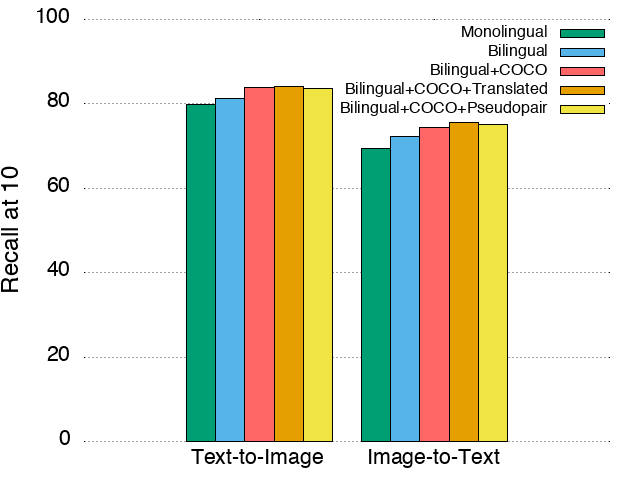
\includegraphics[width=1\textwidth]{assets/best_en_models}
    \caption{English}
  \end{subfigure}%
  \begin{subfigure}[b]{0.5\textwidth}
    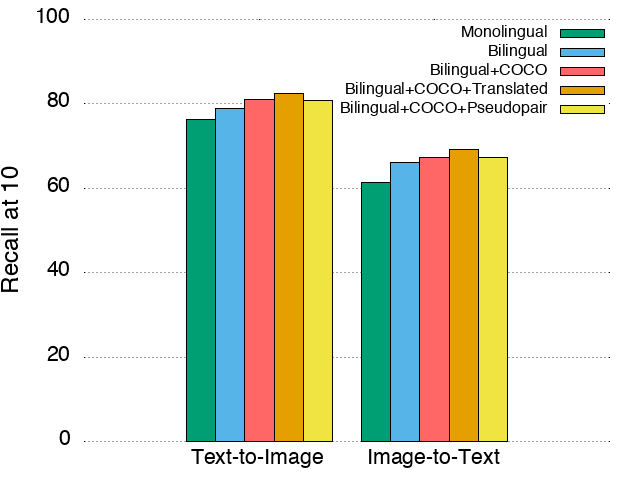
\includegraphics[width=1\textwidth]{assets/best_de_models}
    \caption{German}
  \end{subfigure}
  \caption{A comparison of strategies for training image--sentence ranking models with in-domain and out-of-domain datasets. The Monolingual models are only trained on the Mutli30K English or German data respectively. The Bilingual models are trained on all of the Multi30K data. The +COCO models are trained with the additional English COCO dataset. The +Translated models are trained with German machine translations of the COCO data, and the +Pseudopair models are trained with German annotations transferred from a pre-trained Bilingual model.}
\end{figure*}

\todo[inline]{Include a graph here that shows the absolute best performing models depending on the availability of the data? It would be useful to sum up the findings of this long section.}


%%%
%%%
%%%

\begin{comment}
\section{Experiments}
We consider two main sets of experiments:
%\subsection{THE REAL EXPERIMENTS}
%In the "Lessons learned" paper we had experiments that show that if the images are aligned between languages training joint multilingual models lead to better representations. We had a small experiment showing that disjoint is promising. In this paper our first interest is to see it in a more realistic setting when there is a potential domain mismatch if how does disjoint setting compare. We do not have a large German set so this constrains our experiments. \\

\paragraph{Experiment 1}
We attempt to improve a bilingual English-German image--sentence ranking model by adding a
large external data source. This external source, however, only contains image-English caption pairs. In this experiment, we train our models with English-German Multi30K and then add English-COCO. We use Recall @ 10 performance as the early-stopping criteria, calculated on the validation portion of the Multi30K datasets. \\

\paragraph{Experiment 2: Pseudo pairs}
Follows from Experiment 1. Given a smaller image-German captions dataset and a larger disjoint image-English captions dataset, can we improve performance of the lower-resource German model with the disjoint English dataset? Also, does training with the smaller German dataset affect the performance of the model trained on the larger English dataset? In these experiments, we train on Multi30K-German and English-COCO; early stopping on the Multi30K German dataset. \\

\noindent In both experiments, we test the effectiveness of the pseudo-pair
strategy in the following three settings:

\begin{enumerate}
    \item Constructing pseudo-pairs by Sentence or Image Similarity
    \item Random restart vs. Fine-tuning. Given a new dataset of pseudo pairs, we can either train a model from scratch using the pseudo pairs or use the pseudo pairs to fine-tune the model that was used to extract the pseudo pairs.
    %\item Multiple rounds: the pseudo-pairs can be created after convergence multiple times using the same model.
    \item Caption-to-caption loss: The c2c objective gives an extra dimension to our the experiments. All of the models can be trained with and without this loss c2c objective. When an aligned data set is given (Experiment 1.) we suspect it leads to better quality distant pairs. Furthermore, without an aligned data set between languages (Experiment 2.) the
    pseudo-pairs generate a new caption-caption resource to add the c2c objective. 
\end{enumerate}

%\todo[inline]{What does the third bullet point mean?}


%These two sets of experiments provides us with an initial set of results using the methods we used in the previous "Lessons learned paper". The rest of our effort is then concentrated on improving performance in both setups by finding pseudo-pairs using the models we trained. Our interest here is to use the model itself to bootstrap its own performance without using any external system. 



%\begin{itemize}
%    \item Aligned: We have the aligned M30K German-English. Can we further improve both German and English with adding COCO? Can we further improve German using pseudo-alignments using the learned model?
%    \item Disjoint: We have M30K German and COCO for English. Can we improve both COCO and M30K German results by joint training? Can we further improve further with pseudo-alignments?
%\end{itemize}



\begin{comment}

\subsection{Other stuff}

We evaluate the quality of the sentence representations learned from the  \emph{aligned},
\emph{disjoint} and \emph{distant} data settings on four tasks. In the \emph{aligned} setting, we 
use the comparable portion of the Multi30K data set with 29K images paired with five  English
and five German sentences. In the \emph{disjoint} and \emph{distant} settings, we randomly 
sample 29K images with five English sentences from the COCO data set, and use the five German sentences for the images in the Multi30K data set. 

\paragraph{Image-sentence ranking}
Our intrinsic evaluation to test the quality of the visually grounded sentence representations is retrieving one modality given the other. We report the standard metric recall at 10 (R@10),
but avoid recall at one and recall at five to reduce clutter -- these are also higher variance.
We report the performance on the \emph{comparable} test-set of Multi30K.

\paragraph{Translation retrieval}
We measure the effect of images used as pivots to bridge between languages by retrieving
translation equivalents given the same image. In order to compare out results to previous work, we report precision
at one (P@1) on the \emph{translation} test-set of the Multi30K data set.

\paragraph{Bilingual lexicon induction}
Even though our main goal is to learn multilingual sentence representations the architecture learns multilingual 
grounded word-embeddings as a set of parameters. 
We evaluate how our model compares to approaches developed for bilingual lexicon induction through image-pivoting. We use the word-translation dataset\footnote{Avaliable at \url{https://github.com/coastalcph/cldi_from_image_search/}} introduced in \citet{hartmann2017limitations}.
The data set contains 1,771 word-pairs split into 1,406 nouns, 206 verbs and 159 adjectives. We report standard retrieval based measures: precision at 1 (P@1), 
precision at (P@10), and mean reciprocal rank (MRR).

\paragraph{Natural language inference}
\citet{kiela2017learning} shows that combining visually grounded representations 
with skip-thought vectors leads to improvements on a variety of semantic tasks compared
to the skip-thought only model. In these experiments, we evaluate whether the improvements 
observed in image-sentence ranking through the use of multilingual data sets transfer
outside of the training domain. We use the SNLI and SICK entailment data sets within the SentEval\footnote{\url{https://github.com/facebookresearch/SentEval}} framework. Previous work
trains visually grounded sentence representations on the full COCO data set
\citep{kiela2017learning} and as such we report results with an extra data setting on top of
\emph{aligned}, \emph{disjoint} and \emph{distant}: we use the full COCO for English and the
smaller Multi30K for German leading to \emph{large disjoint} and \emph{large distant} setups.

\subsection{Parameter sharing}

\paragraph{Input representation}
The choice of input representation has a large impact on the amount of parameters the
architecture can share across languages. On the one extreme, for each word in 
the training set a separate embedding is learned, leading to no sharing. 
Remaining on word-level the amount of parameters to be shared can be increased by
learning a single word-embedding for ortographically equivalent words across languages.
% Even more parameters can be shared by considering sub-word encodings such as BPE.
Lastly, on the other end of the spectrum is character-level encoding. For the character-level
model we apply the hierarchical approach: each word is encoded as the last state of 
character-level LSTM whose last hidden-state is fed to the word-level LSTM.

\paragraph{Recurrent parameters (this might not be too much)}
Sharing the whole recurrent-network across languages results in the smallest number of
parameters, however, they might be typological differences between languages that are 
detrimental to the performance of this model. Rather, than experimenting with various 
heuristics we opted for \emph{learning} the parameters to be shared. This is achieved
by the contextual parameter generator network \cite{platanios2018contextual}. It takes
as input a language embedding and generates the parameters for the recurrent network. 
This architecture lets the model learn for itself, which parameters to share across 
languages.

\end{comment}
\end{comment}


\begin{comment}
\begin{table*}[th!]
    \centering
    \renewcommand{\arraystretch}{1.0}
    \begin{tabular}{lcccccc}
        \toprule
         & \multicolumn{3}{c}{I $\rightarrow$ T} & \multicolumn{3}{c}{T $\rightarrow$ I} \\
         & R@1 & R@5 & R@10 & R@1 & R@5 & R@10 \\
         \hline
         \textit{Evaluated on English}\\
         \hline
         English & 40.5  &  69.6  &  79.9   & 28.8 & 58.3 & 69.4  \\
         \; + German & 41.4 & 70.9 & 81.0 & 29.9 & 59.6 & 70.0 \\
         \; + German + c2c & \textbf{42.8} & \textbf{72.0} & \textbf{81.2}  & \textbf{32.1} & \textbf{61.4} & \textbf{72.2}\\
         \hline
         \textit{Evaluated on German}\\
         \hline
         German & 34.9 & 64.1  & 76.2  & 24.6 & 50.1 & 61.3 \\
         \; + English & \textbf{38.6}  & 66.9  &  77.9 & 26.0 & 52.2  & 63.0\\
         \; + English + c2c & 38.3 & \textbf{68.3} & \textbf{78.8} & \textbf{27.7} & \textbf{54.9} & \textbf{66.0}  \\
         \bottomrule
    \end{tabular}
    \caption{German and English Image-to-Text and Text-to-Image baseline results for models trained on only the Multi30K German, German + English, and with the additional caption--caption ranking objective.}\label{tab:baseline}
\end{table*}
\end{comment}

\begin{comment}
\begin{table*}[]
    \centering
    \renewcommand{\arraystretch}{1.0}
    \begin{tabular}{rlcccccc}
        \toprule
         & & \multicolumn{3}{c}{I $\rightarrow$ T} & \multicolumn{3}{c}{T $\rightarrow$ I} \\
         & & R@1 & R@5 & R@10 & R@1 & R@5 & R@10 \\
         1 & German + English + c2c & 38.3 & 68.3 & 78.8 & 27.7 & 54.9 & 66.0  \\
         \hdashline
         2 & COCO + German & 36.4 & 65.9  & 77.6 & 25.7  & 51.6 & 62.6 \\
         3 & \; + English & 39.2  & 67.8  & 79.1 & 27.1 & 53.2  &  64.0  \\
         4 & \; + English + c2c & \textbf{40.6} & \textbf{70.5}  & \textbf{81.1}  & \textbf{28.8} & \textbf{56.3}  & \textbf{67.3} \\
         \bottomrule
    \end{tabular}
    \caption{Results for German models trained with the out-of-domain English COCO dataset. We also include a subset of the baseline models for ease-of-comparison.}\label{tab:coco_en_in_de}
\end{table*}
\end{comment}


\begin{comment}
\begin{table*}[]
    \centering
    \renewcommand{\arraystretch}{1.0}
    \begin{tabular}{rlcccccc}
        \toprule
         & & \multicolumn{3}{c}{I $\rightarrow$ T} & \multicolumn{3}{c}{T $\rightarrow$ I} \\
         & & R@1 & R@5 & R@10 & R@1 & R@5 & R@10 \\
         1 & English & 40.5  &  69.6  &  79.9   & 28.8 & 58.3 & 69.4  \\
         2 & English + German + c2c & 42.8 & 72.0 & 81.2  & 32.1 & 61.4 & 72.2\\
         \hdashline         
         3 & COCO & 34.4  & 61.4  &  72.1 & 24.8 & 50.3  & 61.1\\
         4 & \; + English & 46.2 & \textbf{75.6} & 83.6 & 33.4 & 62.5  & 73.1  \\
         5 & \; + English + German & 46.0  & 75.3 & \textbf{83.9}  & 33.6 & 62.7 &  73.3  \\
         6 & \; + English + German + c2c & \textbf{46.5} & 75.2 & 83.8 & \textbf{34.8} & \textbf{64.4} & \textbf{74.3} \\         
         \bottomrule
    \end{tabular}
    \caption{Results for English models trained with the out-of-domain English COCO dataset. We also include a subset of the baseline models for ease-of-comparison.}\label{tab:coco_en}
\end{table*}
\end{comment}

\begin{comment}
\begin{table*}[]
    \centering
    \renewcommand{\arraystretch}{1.0}
    \begin{tabular}{rlcccccc}
        \toprule
         & & \multicolumn{3}{c}{I $\rightarrow$ T} & \multicolumn{3}{c}{T $\rightarrow$ I} \\
         & & R@1 & R@5 & R@10 & R@1 & R@5 & R@10 \\
         \hline
         1 & Table \ref{tab:coco_en} Best & 46.5 & 75.2 & 83.8 & 34.8 & 64.4 & 74.3 \\         
         \hdashline
         %Translated + English & 42.2 & 71.1 & 80.6 & 30.5 & 57.8 & 68.7 \\ DOESN'T MAKE SENSE
         2 & Translated + English + German & 43.8 & 72.0 & 81.4 & 30.9 & 60.1 & 70.9 \\
         3 & \; + c2c & 44.9 & 73.2 & 82.1 & 33.8 & 61.7 & 72.2 \\
         4 & Translated + COCO + English & 45.6 & 72.9 & 81.1 & 33.0 & 61.0 & 71.8  \\
         5 & \; + German & 46.8 & 74.7 & 83.4 & 33.6 & 62.9 & 73.2 \\
         6 & \; + German + c2c & \textbf{47.5} & \textbf{75.7} & \textbf{84.1} & \textbf{36.2} & \textbf{65.6} & \textbf{75.6} \\  

         %\; + German + c2c & 44.9 & 73.2 & 82.1 & 33.8 & 61.7 & 72.2 \\
         %\; + German + COCO & 46.8 & 74.7 & 83.4 & 33.6 & 62.9 & 73.2 \\
         %\; + German + COCO + c2c & \textbf{47.5} & \textbf{75.7} & \textbf{84.1} & \textbf{36.2} & \textbf{65.6} & \textbf{75.6} \\  
         \bottomrule
    \end{tabular}
    \caption{Results for English models trained with the machine translation-generated German captions for the COCO dataset. We also include the best performing English model from Table \ref{tab:coco_en} for ease-of-comparison.}\label{tab:coco_en-mt}
\end{table*}
\end{comment}

\begin{comment}
\begin{table*}[]
    \centering
    \renewcommand{\arraystretch}{1.0}
    \begin{tabular}{rlcccccc}
        \toprule
         & & \multicolumn{3}{c}{I $\rightarrow$ T} & \multicolumn{3}{c}{T $\rightarrow$ I} \\
         & & R@1 & R@5 & R@10 & R@1 & R@5 & R@10 \\
         \hline
         1 & COCO + German + English + c2c & 40.6 & 70.5  & 81.1  & 28.8 & 56.3  & 67.3 \\
         \hdashline
         2 & Translated + German & 38.5 & 68.4 & 79.6 & 26.6 & 53.7 & 64.4\\
         3 & \; + COCO & 39.1 & 69.8 & 80.2 & 27.5 & 54.2 & 64.7 \\
         4 & \; + English & 39.8 & 69.6 & 81.0 & 27.6 & 54.8 & 65.5 \\
         5 & \; + English + c2c & 38.2 & 66.3 & 77.0 & 27.2 & 54.2 & 65.5 \\
         6 & \; + COCO + English & 40.2 & 71.2 & 81.9 & 28.3 & 55.6 & 66.1 \\
         7 & \; + COCO + English + c2c & \textbf{43.5} & \textbf{73.3} & \textbf{82.5} & \textbf{30.5} & \textbf{58.8} & \textbf{69.3} \\         
         \bottomrule
    \end{tabular}
    \caption{Results for German models trained with the machine translation-generated German captions for the COCO dataset. We also include the best performing model from Table \ref{tab:coco_en} for ease-of-comparison.}\label{tab:coco_de-mt}
\end{table*}
\end{comment}
